\documentclass[12pt,letterpaper,titlepage]{article}
\usepackage[left=1.00in, right=1.00in, top=1.00in, bottom=1.00in]{geometry}
\usepackage{times}
\usepackage{graphicx}
\usepackage{listings}
\usepackage{float}
\usepackage{url}
\setcounter{secnumdepth}{4}
\setcounter{tocdepth}{4}
\setlength\parindent{12pt}
\begin{document}
	\title{ME 382 ASME Design Competition Final Report}
	\date{ Team: 10-6 \\
		\bigskip
		20 March 2017 \\
		\medskip	
		Presented for Dr. Hoyle and Vincenzo Ferrero}
	\author{Matthew Hoeper
		\and Nathan Imholt
		\and Brandon Low
		\and Jake Peden
		}
		
	
	\maketitle
\graphicspath{{.images/}}
\tableofcontents
\listoffigures
\pagebreak
\section{Introduction}
%%%
This report is a final write up for team 10-6's design process and results for the ASME Design competition for ME 382 in winter term, 2017. For Winter 2017, the design competition was modified to have 4 distinct problems. A vehicle that is operated via controller must be able to drive 5 meters, pick up a ping pong ball, drive back, climb small stairs, and finally shoot the ping pong ball 3 meters. The project was undertaken by our team in order to satisfy class requirements and thereby graduation requirements as well as personal gain. As defined in our Team Charter the two goals our team had were to finish in the top 10 and for everyone to earn a B or better. There were a few restrictions imposed on the end product. Namely, the product must fit in a 50x50x50 cm box and all energy must come from rechargeable batteries. The project began in the first week of January and the field test took place on the 16th of March. A hard limit of 10 weeks was a severely limiting factor because any sort of delay will have an effect on the time line of everything there after. Essentially, if the overall design was non functional after assembly there was not an opportunity to amend it. Another logistical limitation was budget. The entire project must be completed with \$200 excluding the controller.  
%%%
\section{Design Approach}

This section is the most extensive aspect of this report. It covers all the areas that were covered in class and were written about in the project update memos. The design approach was derived from Dr. Ullman's book, \textit{The Mechanical Design Process.} Our approach encompasses 5 of the 6 areas of the design process; Product Discovery, Planning, Definition, Conceptual Design, Development. Support is excluded because there is no end of life support \cite{textbook}. 

\subsection{Project Plan}
\textbf{Introduction} 

The purpose of this section is to cover our team's project planning process and how we equally divided up the work. The section contains three subsections, the purpose of project planning, where we describe the purpose of project planning, the approach, a description of our approach to project planning, and the results which is a Gantt Chart we generating from our first meeting. As well as a discussion of what we learned during the meeting. 

\smallskip\noindent\textbf{Purpose of Project Planning} 

The purpose of project planning is to understand the scope of the project set in front of the team. Project planning allows us to look at the project as a whole and the deliverables tasks that must be completed and break them down into individual assignable substeps. This helps us develop a rough time frame and a basic structure for work. By having the project mapped out it allows for more flexibility in the event that a task goes astray because we can see how much a single task will affect the remaining ones. 

\smallskip\noindent\textbf{Approach} 

The approach my team took to project planning was to create a WBS first and lay out tasks and the associated steps thoroughly so we were aware of what events needed to take place for us to compete in week 10. We then used the larger tasks as the events in a Gantt Chart (see Figure 1). Comparing the difficulty of the individual substeps associated with larger tasks we used personal experience with projects to estimate a time frame. After deciding the events present in the Gantt Chart, we laid out the critical path and marked it in red. Critical path events were designated as such because we thought they were impassible events. We assigned design responsibilities to teams of two based on experience and in an attempt to keep the workload off a single person. Other tasks that are simple enough for a single person to do would have a member of the team volunteer and take responsibility for it. The final tasks that were large and required the effort of every team member were noted as such and will require a group effort as they are completed. 

\smallskip\noindent\textbf{Results}

One of the results of project planning is a clearer picture of the process we have to use in order deliver a capable robot at the end of the term. This process helped us create a Gantt Chart to keep track of how on or off time we are. 

\begin{figure}[h]
	\centering
	\includegraphics[width=\textwidth]{images/WBS}
	\label{fig:WBS}
	\caption{Gantt Chart}
\end{figure}

\smallskip\noindent\textbf{Discussion}

The findings of this process are the Gantt Chart and the WBS structure. The WBS was instrumental in the development of  a realistic timeline and the development of a Gantt Chart. The Gantt Chart was the best way to divide up work and look at the critical tasks in designing and manufacturing the robot. We learned that by sitting down and planning out the design process before diving straight into it you save time in distributing work and save time that would be spent prioritizing events in case a timeline is not met. 

\pagebreak
\subsection{Customer Requirements and Engineering Specifications}
\smallskip\noindent\textbf{Introduction}

The purpose of this section is to describe how our team used the House of Quality to form specific goals for our project and how we related customer requirements to engineering specifications. This section is divided into four subsections describing what a house of quality is, how we used it, and the results we got after creating our House of Quality.

\smallskip\noindent\textbf{Purpose of HoQ}

The house of quality (HoQ) is a table designed to take qualitative and quantitative customer requirements (CR's) and turn them into quantitative engineering specifications (ES's). It also prioritizes the ES's based on customer weight, how closely they relate to CR's, and the predicted difficulty in meeting the goals of each ES. Specific targets for each ES are formed in the HoQ along with the acceptable design range for those targets, how each ES will affect other ES's, and how they can be optimized.

\smallskip\noindent\textbf{Approach}

Our team started the HoQ by first carefully reading over the competition rules and guidelines. The competition rules lead to the majority of our CR’s. For example, size specifications and the ability to pick up and throw a ping pong ball are both laid out in the rules so they are reflected in our CR’s (Figure 2). We used those requirements to think of what ES’s would lead to fulfilling those requirements. Some targets were harder to come up with than others such as battery life. Since we did not know what kind of power demands the project would need, we had to estimate what kind of battery life seemed appropriate (Figure 2). The maximum dimensions of our robot are provided in the competition rules so our target is to be within those given dimensions. There were also a number of ES’s that were applicable to multiple CR’s and vice versa. For example, torque, tire size, and weight all contributed to climbing ability.

\smallskip\noindent\textbf{Results}

The house of quality made us realize just how critical weight control was. Most of the negative relationships between ES’s were to do with weight (e.g. more battery life means more weight, more weight means more difficult to climb stairs) (Figure 2). It’s important to note that the ES for dimensions (Figure 2) is ranked the highest because without it the rest of competition would be null. Coming in second is Torque which will dominate the sprint and climbing portions of the competition. In the ES vs. ES section, weight has 5 negative relations with other ES’s (Figure 2). The tradeoff between weight and a high performance design will be an important thing to consider going forward. 

\begin{figure}[h]
	\centering
	\includegraphics[width=5in]{images/HOQ-1}
	\label{fig:HOQ}
	\caption{House of Quality}
\end{figure}


\smallskip\noindent\textbf{Discussion}

Through the ES rankings we found that throughout the design process we need to focus on keeping the dimensions to below 50 cm in any direction and having sufficient torque. Additionally, weight will need to be accounted for large systems even though there is no weight restriction. We also found that we don't necessarily need to focus on battery life and having a strong chassis. These findings correspond with the nature of the competition rules. Our most important specifications are directly related to the functions stated in the competition rules. The least weighted specifications are items that we want rather than need, like long battery life or chassis strength; we are able to change batteries between events. Most materials that are considered for a project of this scale generally should provide enough strength.

\subsection{Functional Model}

\smallskip\noindent\textbf{Introduction}

The intended purpose of this section is to provide an insight to our team's functional model for our robot and the design options that make up each subsystem. Both a Level 0 and a Level 1 model are included. The approach we took towards the functional model as well as the specific results will be also be discussed. 

\smallskip\noindent\textbf{Purpose of a Functional Model}

The intended purpose of a functional model is to have a graphical representation of a system’s function and subfunctions. The way each function and subfunction interact with energy, materials, and signals are outlined in the functional model as a way to conceptually link each sub function with one another. This methodology allows us to more accurately design subsystems that can integrate with one another. 

\smallskip\noindent\textbf{Approach}

The overall approach we used to build our functional model was to start with a black box model. This is the Level 0 section (Figure 1). The condensed single function of the project is laid out explicitly. We assumed that an RC controller would be used to control it. To break down the overall function of the robot we sketched out a broad functional model that incorporated each one of the subsystems. The subsystems include propulsion, ball pick up, ball throw, electrical, and control. Customer requirement are what drove the initial subfunctions in each chain. As the chain progressed the further the customer requirement were able to describe the functions. To finalize the functional model we broke down each subsystem into as many subfunctions as there are design challenges. The flows were determined by writing down what each subfunction needs to operate and deciding where the needs would be drawn from. Energy loss flows were included even though the robot can't utilize them.

\smallskip\noindent\textbf{Results}

Two of our customer requirements, completing the course without human input and use electrical energy, dominate the functional model. Upon the completion of the functional model we had a distinct representation of how the electrical system applies to everything (Figure 3). Prior we had no real idea of how the electricity would be distributed to each system. Another thing to note is that for every sub function that has electrical energy and an electrical signal there needs to be some sort of electrical component such as a relay to make sure not every subfunction is not running all the time. The only sub function  that is independent of anything else besides electrical energy and signal is 'Aim Shooter'  in Figure 3. This is because we want to be able to do this whether or not anything else is running; it needs to be an unconstrained function.
\begin{figure}[H]
	\centering
	\frame{\includegraphics[width=4.65in]{images/FuncModel}}
	\label{fig:Func}
	\caption{Functional Model}
\end{figure}

\smallskip\noindent\textbf{Discussion}

We are now aware of how complicated the control system is going to be. Whether or not each subfunction of will have to be it's own device or incorporated into some sort of code is something that will have to be investigated further. Our functional model was created with the ability to either have the shooting system run completing autonomous or by using human intervention. If the our design concepts permit, we will attempt to have pick up and shooting system integrate seamlessly. 

\subsection{Concepts}

\smallskip\noindent\textbf{Introduction}

The purpose of this section is to describe our team's concept generation and screening process. This section contains three subsections, the purpose of concept screening in which we describe why we went through the concept screening process, an approach section where we go into detail about how we went about generating concepts and the criteria we used to score them, as well as a results section that outlines what we discovered after having scored all of our concept variants. There is also a discussion section where we talk about what we learned during this process.

\smallskip\noindent\textbf{Purpose of Concept Screening}

The concept screening process utilizes a certain kind of matrix called a Pugh Chart. This chart allows our group to see all of the concept variants that we have come up with, decide on a datum design that the rest of the concept variants will be scored against, and finally analyze each design in depth and decide whether they would perform better or worse when compared to the datum. 

\smallskip\noindent\textbf{Approach}

Before starting with the Pugh Chart our group first started with a morphological matrix that consisted of the sub functions described in our functional model as well as our proposed solutions to each of these sub functions. After we had completed this chart we took one solution for each sub function and created a robot design that could fulfill all of the required functions (10 total). The first concept (Figure 5) was derived from the rough designs that we had already been thinking about from the first few weeks of the project. Both the second and third concepts (Figure 5 and 6 respectively) were put together with what we thought would be the next best concepts from the different pieces of the morphological matrix. We then put these concepts along with the 6 others into the Pugh Chart (Figure 4) and scored 6 of them against the one datum concept that we had selected as the most optimized design. The concepts were given a minus (-) if they would perform lower than the datum, a plus (+) if they would reform better and a 'same' (S) score if the variant was the same as the datum concept.

\smallskip\noindent\textbf{Results}

After completing the screening process, we noticed that many of the concepts that we had come up with had mostly sminus' and 'same' scores, this is evident in the totals at the bottom of the Pugh Chart (Figure 4) where all of the nine designs have relatively low 'plus' totals. We expected this result since the datum (Figure 5) was the concept that we came up with first and we tried to optimize the first concept to best match what we thought was feasible for us to build and operate. Since the scores were relatively low the second and third concept variants (Figures 5 and 6 respectively) most likely wont be our choices for final designs. The second concept includes a complex claw mechanism to pick up the ping pong ball, this claw would be difficult to manufacture and would end up being difficult to control. The third concept has four motors, tank treads and an aluminum chassis; making it the heaviest and most expensive design.
\begin{figure}[H]
	\centering
	\includegraphics[height=3.5in]{images/CVscreen}
	\label{fig:CVscreen}
	\caption{Pugh Chart}
\end{figure}

\begin{figure}[H]
	\centering
	\includegraphics[width=4in]{images/CV1}
	\label{fig:CV1}
	\caption{Concept Variant 1}
\end{figure}

\begin{figure}[H]
	\centering
	\includegraphics[width=4in]{images/CV2}
	\label{fig:CV2}
	\caption{Concept Variant 2}
\end{figure}

\begin{figure}[H]
	\centering
	\includegraphics[width=4in]{images/CV3}
	\label{fig:CV3}
	\caption{Concept Variant 3}
\end{figure}




\subsection{Design Analysis}
\smallskip\noindent\textbf{Analysis Method 1: Trajectory}

\medskip\noindent\textbf{Purpose}

This analysis method was used to find the ideal angle of fire and a given initial velocity provided by the air cannon. The ODE solver was created to incrementally increase the angle of fire and to accurately find the optimal velocity needed to reach a 3 meter distance. 

\medskip\noindent\textbf{Analysis}

The solver was derived from a bi-directional force balance that included drag in both the x and y axes. The x direction is distance in which the target lies in relation to the stairs. The y direction is vertical distance from the target height. The initial velocity and angle would be manually entered and then iteratively change to search for the optimal set of conditions. The initial y height is given by the height of the stairs plus the height of the barrel from the stairs. We started with putting vectors for both velocity and angle and slowly finalized a few. The following code has the script first and then the function that conditions ode45 for Matlab. The initial conditions in the code below are are the final set we found by incrementally increasing theta by 5 degrees from 0. The first angle is 0.5 degrees because the ball would roll out if it were actually 0. 


\bigskip\noindent\textbf{ODE Solver:}

\begin{lstlisting}[language=matlab]
clear all;clc
vi = [15 10.15 8.95 8.1 7.0]; % input inital velocity here
theta = [0.5 5 7.5 10 15] ; % angle of fire
for j = 1:length(vi)
for i = 1:length(theta)
i = j;
x0 = 0;
vx0(i) = vi(j)*cosd(theta(i)); % optimal is 9.88 m/s with 1 m/s in y: 5 degree angle
y0 = 0.15+(5.9/2.54)/100;  % height of stairs  plus robot
vy0(i) = vi(j)*sind(theta(i));
IC = [x0 vx0(i) y0 vy0(i)];

[t,z] = ode45('Pong', [0 1.5], IC);
plot(z(:,1),z(:,3)); grid on; hold on
axis([0 3.5 0 0.5]);
xlabel('x (m)')
ylabel('y (m)')
ref = refline(0,0);
ref.LineStyle = '--';
ref.Color = 'k';
end
end

function dzdt = Pong(~,z)
rho = 1.10;
A = pi*(40/1000)^2;
Cd = 0.47;
k = -1/2*rho*Cd*A;
m=0.003;
v = sqrt(z(2)^2 +z(4)^2);
dzdt(1)= z(2);
dzdt(2)= k*z(2)/v^2/m;
dzdt(3)= z(4);
dzdt(4)=(k*z(4)/v^2)/m-9.81;
dzdt = dzdt';
end
\end{lstlisting}
\bigskip
\bigskip

\begin{figure}[H]
	\centering
	\includegraphics[width=\textwidth]{images/ODE}
	\label{fig:ODE}
	\caption{Varying trajectories of a ping pong ball}
\end{figure}

\smallskip\noindent\textbf{Results}

As seen in Figure 8, after using the Matlab script and function, the four best sets of conditions are 5 degrees with 10.15 m/s, 7.5 degrees with 8.95 m/s, 10 degrees with 8.1 m/s, and 15 degrees with 7.0 m/s. These results are essential because now we can program a specific angle for a servo to go to. Then we can roughly estimate how much pressure is needed to reach a velocity and experimentally determine the necessary pressure for that. 


\bigskip\noindent\textbf{Analysis Method 2: Time to fill the pressure vessel}

\medskip\noindent\textbf{Purpose}

This analysis was a calculation to determine the maximum amount of time the air compressor will have to run in order to fill the pressure vessel to the the highest pressure the compressor can run up to. This calculation was necessary to make sure our shooting device would complete in under two minutes. 

\smallskip\noindent\textbf{Analysis}

A few assumptions were made in order to carry out the analysis. The first being that air is an ideal gas and the initial pressure of vessel was at standard atmospheric pressure. The second assumption was that the compressor operated at steady state at all times; this assumption may be too forgiving because the compression rate may slow down as the pressure increases. The last assumption is that the temperature of air is constant across the compression process. The volumetric flow rate was given by the manufacturer at a rate of 0.35 cubic feet per minute \cite{compressor}. The initial mass at STP was found and the final mass at maximum pressure. Then the volumetric flow rate was converted to a mass flow rate. Time to fill was found by subtracting final mass from initial mass and dividing by mass flow rate. 
\smallskip

\begin{figure}[H]
	\centering
	\includegraphics[width=\textwidth]{images/fill}
	\label{fig:fill}
	\caption{Written analysis of the pressure vessel filling time}
\end{figure}


\smallskip\noindent\textbf{Results}

With the air compressor that we chose to use for the competition, it will approximately take 32 seconds to fill the pressure vessel to the maximum pressure possible according to the analysis in Figure 9. Since we have two minutes to fire then we will have plenty of time to fill the pressure vessel, fire and even return to maximum pressure. The actual time we will spend filling may be even less as maximum pressure may not be necessary for the target distance.

\bigskip\noindent\textbf{Analysis Method 3: Force need to pick up ball}

\medskip\noindent\textbf{Purpose}

This method is another calculation to find out if a 120mm PC fan can create a large enough pressure differential to lift the ping pong ball up off the ground at an ample speed. 

\smallskip\noindent\textbf{Analysis}

This analysis was carried out using a simple force balance to determine the pressure needed to suspend the ping pong ball. The area in which the pressure force acted was assumed to be half of the surface area of the ball. We were originally going to use this assumption at first then find the necessary pressure and if they were too close we would re evaluate the assumption. To find the pressure differential conservation of mass and Bernoulli's equation was used. The volumetric flow rate of the fan was specified by the manufacturer to be 70 cubic feet per minute (Rosewill, Inc, 2015) Mass flow rate of the air was found using volumetric flow rate. Once the mass flow rate was found, the velocity of air was calculated and plugged into Bernoulli's equation to find the pressure differential. 

\begin{figure}[H]
	\centering
	\includegraphics[width=\textwidth]{images/ballpickup}
	\label{fig:pickup}
	\caption{Force and pressure balance on the Ping Pong Ball}
\end{figure}

\smallskip\noindent\textbf{Results}

The calculations in Figure 10 show that we need a baseline pressure difference of at least 21 pascals to balance the force of gravity acting on the ball. We determined that the fan can create a pressure difference of 160 Pascals, more than enough to pick up the ball. The volumetric flow rate was a mid level fan; some fans have an even higher flow rate so this design is solid. 

\bigskip\noindent\textbf{Analysis Method 4: Torque in barrel servo}

\medskip\noindent\textbf{Purpose}

For this method we used a calculation spreadsheet in Excel to determine the moment that the barrel and fan will exert on the servo it's mounted to. The moment will tell us the necessary torque the servo must output for steady and quick rotation. 

\smallskip\noindent\textbf{Analysis}

The density, volume and mass values were directly transcribed from the mass properties function in Solidworks. These values will be extremely accurate as the shroud will be 3-D printed so the Solidworks model will directly reflect the physical product. The moment was calculated in kg-cm because many servo data sheets have torque specified in kg-cm or oz-in. 

\begin{figure}[H]
	\centering
	\includegraphics[width=\textwidth]{images/MomentServo}
	\label{fig:MomentServo}
	\caption{Moment arm calculation in Excel}
\end{figure}

\smallskip\noindent\textbf{Results}

The calculation shows that the servo we use to pitch the barrel up and down will need to be able to rotate with an induced moment of 4 kilograms centimeter as can be seen in the dark green box (Figure 11).

\bigskip\noindent\textbf{Analysis Method 5: Layout}

\medskip\noindent\textbf{Purpose}

For this analysis our group used a Solidworks assembly to incorporate all of the models we created for the various parts. We used Solidworks so that we could accurately plan the layout for the robot, as well as make adjustments to how we were planning on mounting each part.

\smallskip\noindent\textbf{Analysis}

In order to effectively create a layout we either downloaded a pre existing model from a manufacturer or used calipers to model the part ourselves. We started with a chassis that was slightly undersized the 50cm x 50cm requirement to make sure the width of the tires were accounted for. Then we added the models and created a few different layouts until we were comfortable with the design. Smaller components such as wires, fittings or hoses were exempt from the model because the are not static and can be moved to accommodate larger components.  

\smallskip\noindent\textbf{Results}

The models in Figures 12 through 15 show that all of the parts we are using will fit well on the robot. We also wanted to make sure that we would still have enough space in between the parts to integrate them all correctly with wire and tubing. The distance from the back side of the chassis to the most forward part of the barrel is roughly 48 cm so we have some extra room. At the widest, the robot is about 48 cm as well. The tallest part of the robot is well under 50 cm so there should be no issue in fitting in the sizing box. 

\begin{figure}[H]
	\centering
	\includegraphics[width=3.6in]{images/layout1}
	\label{fig:layout1}
	\caption{Isometric view of assembly}
\end{figure}
\begin{figure}[H]
	\centering
	\includegraphics[width=3.6in]{images/layout2}
	\label{fig:layout2}
	\caption{Bottom view of assembly}
\end{figure}
\begin{figure}[H]
	\centering
	\includegraphics[width=3.5in]{images/layout3}
	\label{fig:layout3}
	\caption{Right view of assembly}
\end{figure}
\begin{figure}[H]
	\centering
	\includegraphics[width=3.5in]{images/layout4}
	\label{fig:layout4}
	\caption{Rear view of assembly}
\end{figure}


\subsection{Design for Manufacture and Assembly}

\smallskip\noindent\textbf{Introduction}

The purpose of this section is to describe how our team went about estimating the assembly time of our robot, as well as a description of the design for an assembly checklist. The section contains three subsections; the purpose where we discuss why we worked through the DFA and DFM, an approach section where we talk about how we made our decisions in the tables, and a results section containing what we found out during this process. The two worksheets we used were adapted from Dr. David Ullman's book \cite{textbook}. There is also a discussion section at the end where we talk about future steps for the project.

\smallskip\noindent\textbf{Purpose of DFA/ Assembly Estimate}

The purpose of the design for assembly table (Figure 16) is to score our design on ease of assembly, it also shows us where our assembly can be improved for the most efficient building process. The assembly time estimation (Figure 17) is used so that we can foresee how much time we will have to spend actually building the robot once we have all of the parts we need. This allows us to plan a latest start date for assembling the robot so we can finish in time for the competition.

\smallskip\noindent\textbf{Approach}

The approach we took for the assembly time estimation (Figure 17) was to start with listing out all of the processes that we would have to complete to completely assemble the robot. Since we had already done some of the assembly work before hand we used the time it took to build those components to estimate the time it would take to complete the rest of the robot. We chose to exclude certain manufacturing from the estimation such as 3D printing. The steps were determined upon subassembly and sub function. Parts relating to shooting or storing air were bundled. Other concept variants were neglected because it was fairly late in the term and we had finalized our design. As for the DFA (Figure 16) we looked at all of the parts that we in our CAD model and the bill of materials in order to complete the table, analyzing the number of parts and the types of parts we had and scored our design accordingly. 

\smallskip\noindent\textbf{Results}

For the DFA table we found that since the project is small in scale and efficiency of assembly wasn't our first priority we scored low on some of the criteria than what would be expected for an industry project. For example in the DFA table (Figure 16) under “minimum use of separate fasteners” we got a score of 0 since all of the parts will be secured to the chassis with bolts/nuts or wood screws. We also got a score of 0 on the “chamfers and self alignment” category because everything we are building or using is at right angles. The only exception is the slot for the fan shroud. We scored high in the “maximum part accessibility” and “assembly stability” categories since the entire robot is built off of a flat piece of plywood it is easy to get to each part even when they're fastened to the chassis since we haven't made a body to fit over the robot.

For the assembly time estimate (Figure 17) we found that the longest assembly jobs would be mounting the barrel servo sub assembly, mounting the wheels, assembling the pressure vessel, and wiring the circuit. Both the barrel subassembly and the wheel mounting steps have several parts that need to be machined so they take up significant time. The pressure vessel will take 45 minutes because it must be clamped or held down for the epoxy to cure sufficiently. Wiring the robot will require us to test the electrical functions of each part and making sure they all work properly when receiving signals from the controller. The total time of the ideal assembly is 260 minutes. However, it's important to note that the time is for an ideal case, assuming all of our design parts work and integrate as well as we think they will.

\begin{figure}[H]
	\centering
	\includegraphics[width=5.25in]{images/DFA}
	\label{fig:DFA}
	\caption{Design for Assembly Scoring}
\end{figure}

\begin{figure}[H]
	\centering
	\includegraphics[width=5.25in]{images/AssemTime}
	\label{fig:AssemTime}
	\caption{Assembly Time Estimation (minutes)}
\end{figure}

\smallskip\noindent\textbf{Discussion}

Our results from the assembly time estimate helped show us that we are on time to finish the robot before the competition assuming no major problems arise. We will also have enough time to test each of the functions thoroughly. Our design is solid overall; mostly everything works well. The compressed air system isn't powerful as we thought, but it should still provide ample energy for shooting the ball. The DFA table showed us that our assembly method and design is not efficient and would not scale well for mass production. If we were creating this design for mass production we would most likely look for a better way to fasten the parts to the chassis while reducing the number of actual fasteners used. An important design change we could make is to combine a few of the parts for the barrel subassembly. We designed them around smaller parts because we figured we would be limited by what scrap was available in the machine shop. We would also look for parts with smaller versions to reduce the size of the entire robot and eliminate extraneous material.

\subsection{Failure Mode and Effect Analysis}

\smallskip\noindent\textbf{Introduction}

The purpose of this memo is to describe how our team went about evaluating the various modes of failure for the robot and how they would affect the overall function of the robot. The memo contains three sections. The purpose where we discuss why failure mode analysis is necessary, an approach section where we talk about how we made our decisions in the table, and a results section containing what we found out during this process. There is also a discussion section at the end where we talk about future steps for the project.

\smallskip\noindent\textbf{Purpose of FMEA}

FMEA is a process used to determine what parts of any given design are most likely to fail, what would cause this failure, and what measures can be taken to help reduce the chance of failure or mitigate the effects of a possible failure. The end goal of FMEA is that the design team would both think of new failure modes that haven't already been accounted for in the design, as well as take a closer look at how current weaknesses in the design can be fixed. The FMEA also gives contingency plans for the failures that are either more likely to happen or would have the biggest negative effect on the design.

\smallskip\noindent\textbf{Approach}

To start we first broke up the design into 5 major areas: electrical components, completing the sprint, picking up the ball, throwing the ball and climbing up the stairs. After we separated the possible areas of failure we focused on how each function could conceivably fail. We used some of the difficulties we were having in assembly along with observations made during the building process to come up with most of the failure modes. Once the failure modes and their effects were determined we moved on to scoring the severity of the failures, how likely it would be for each to occur, and how our design mitigates these failures. All of the scores we gave were based on a 1 to 10 scale, for the “severity” and “occurrence”, 10 being very severe/ likely to occur. This is different than what was presented in class. The occurrence is based on how often a failure occurs in 100, 1000, or 10000 products. Since the class is not based around mass assembly we went with a more arbitrary scale. For the deterrent column the scale was still 1 to 10 but the score was higher if there are no current designs to mitigate the possible failure modes. Per, Dr. Hoyle, if the product of the three scores was over 100, we needed to come up with an action that can mitigate the possible failure, after the action was taken we could re-evaluate the three scoring criteria and see how the action affected the score.

\smallskip\noindent\textbf{Results}

The FMEA table gives us a comprehensive look at all of the ways our robot could fail, there were only three failures that scored high enough to require further action beyond the testing and refining that we would do during and after assembly. A blank box for “Failure Mode” or “Failure Effect” means it is the same as the one above it. Two of these failure modes, failure of motor controllers and pressure vessel leaking, have been resolved in the “Actions Taken” tab (Figure 1).  The third failure mode, not enough air delivered to barrel, will require some testing to see if the amount of air lost is enough to affect the function of the shooting. The other failure modes can be avoided through careful assembly and testing of the final robot. Failures involving vibration or electrical issues are going to be avoided by taking a close look at each assembly step as well as careful testing of the circuitry of the robot before all of the components are fastened into their final positions so that preventative measures can be taken. The results also show us that the function with the lowest chance of failure is the pick up mechanism. This is to be expected because it is an extremely simple design. 

\begin{figure}[H]
	\centering
	\includegraphics[height=6.35in, width=6in]{images/FMEA}
	\label{fig:FMEA}
	\caption{Failure Mode and Effect Analysis}
\end{figure}

\smallskip\noindent\textbf{Discussion}

Motor controller failure will be easily avoided by using 30A fuses. The 30A value comes from the fact that the motors can draw up to 25A \cite{car seat motor} but the motor controller can withstand 43A \cite{motor driver}. A value in the middle seemed appropriate. The leaking pressure vessel is going to mitigated by the use of RTV silicone sealant. It's vicious when applied but hardens a bit; it's used for high pressure and high temperature sealing in automobiles. We can look down our list of design controls, using it as one of the final checks, to make sure that we've taken every measure to ensure the robot has the highest success rate possible. Our design didn't score very well in some of the shooting functions, this is to be expected since the shooting mechanism is the most complicated part of the design and has a higher degree of uncertainty due to this complexity. These two modes along with the possible motor controller failure will need to be heavily tested once the robot is completed to determine whether we need to take action or not, especially for the shooting mechanism. Failure modes that score upwards of 80 are still important to keep track of such as, chassis snaps due to high impulse, or motor doesn't apply torque to wheels. This is because while these failures have a low chance of occurring they can be catastrophic and could set our team back a few days. 

\section{Bill of Materials}
\begin{figure}[H]
	\centering
	\includegraphics[width=\textwidth]{images/BOM}
	\label{fig:BOM}
	\caption{Final Bill of Materials}
\end{figure}

The above bill of materials is inclusive of everything used on the robot except for adhesives such as tape or epoxy and paint. All aluminum and HDPE used was priced out as scrap because it was found in the machine shop. It's important to note that the most expensive aspect of the robot is the electromechanical side coming in at around \$85.



\section{Results}

The results of the field test went well when compared to our initial goal. We ended up in a three way tie for 6th place out of the 24 competitors. Our initial goal was to place in the top ten, so this was fantastic achievement for us. Unfortunately, as we designed and built the robot we had thoughts of finishing higher. We likely would have if we didn't run into problems on stage. One of our motors wound up with a loose connection which left us unable to do the sprint, pickup, or climb events. We were, however, still able to shoot the ball and our accuracy alone got us sixth place. We were mostly disappointed at being unable to perform all of the tasks. In short, our design uses a pitch-able barrel with a PC fan that generates enough pressure to suck the ball up. The barrel is then pitched back up, an air compressor is ran with the air being stored in the black pressure vessel. The firing mechanism is a modified sprinkler valve where the air is fed into the barrel via plastic tubing. Below are a few pictures of the robot.

\begin{figure}[H]
	\centering
	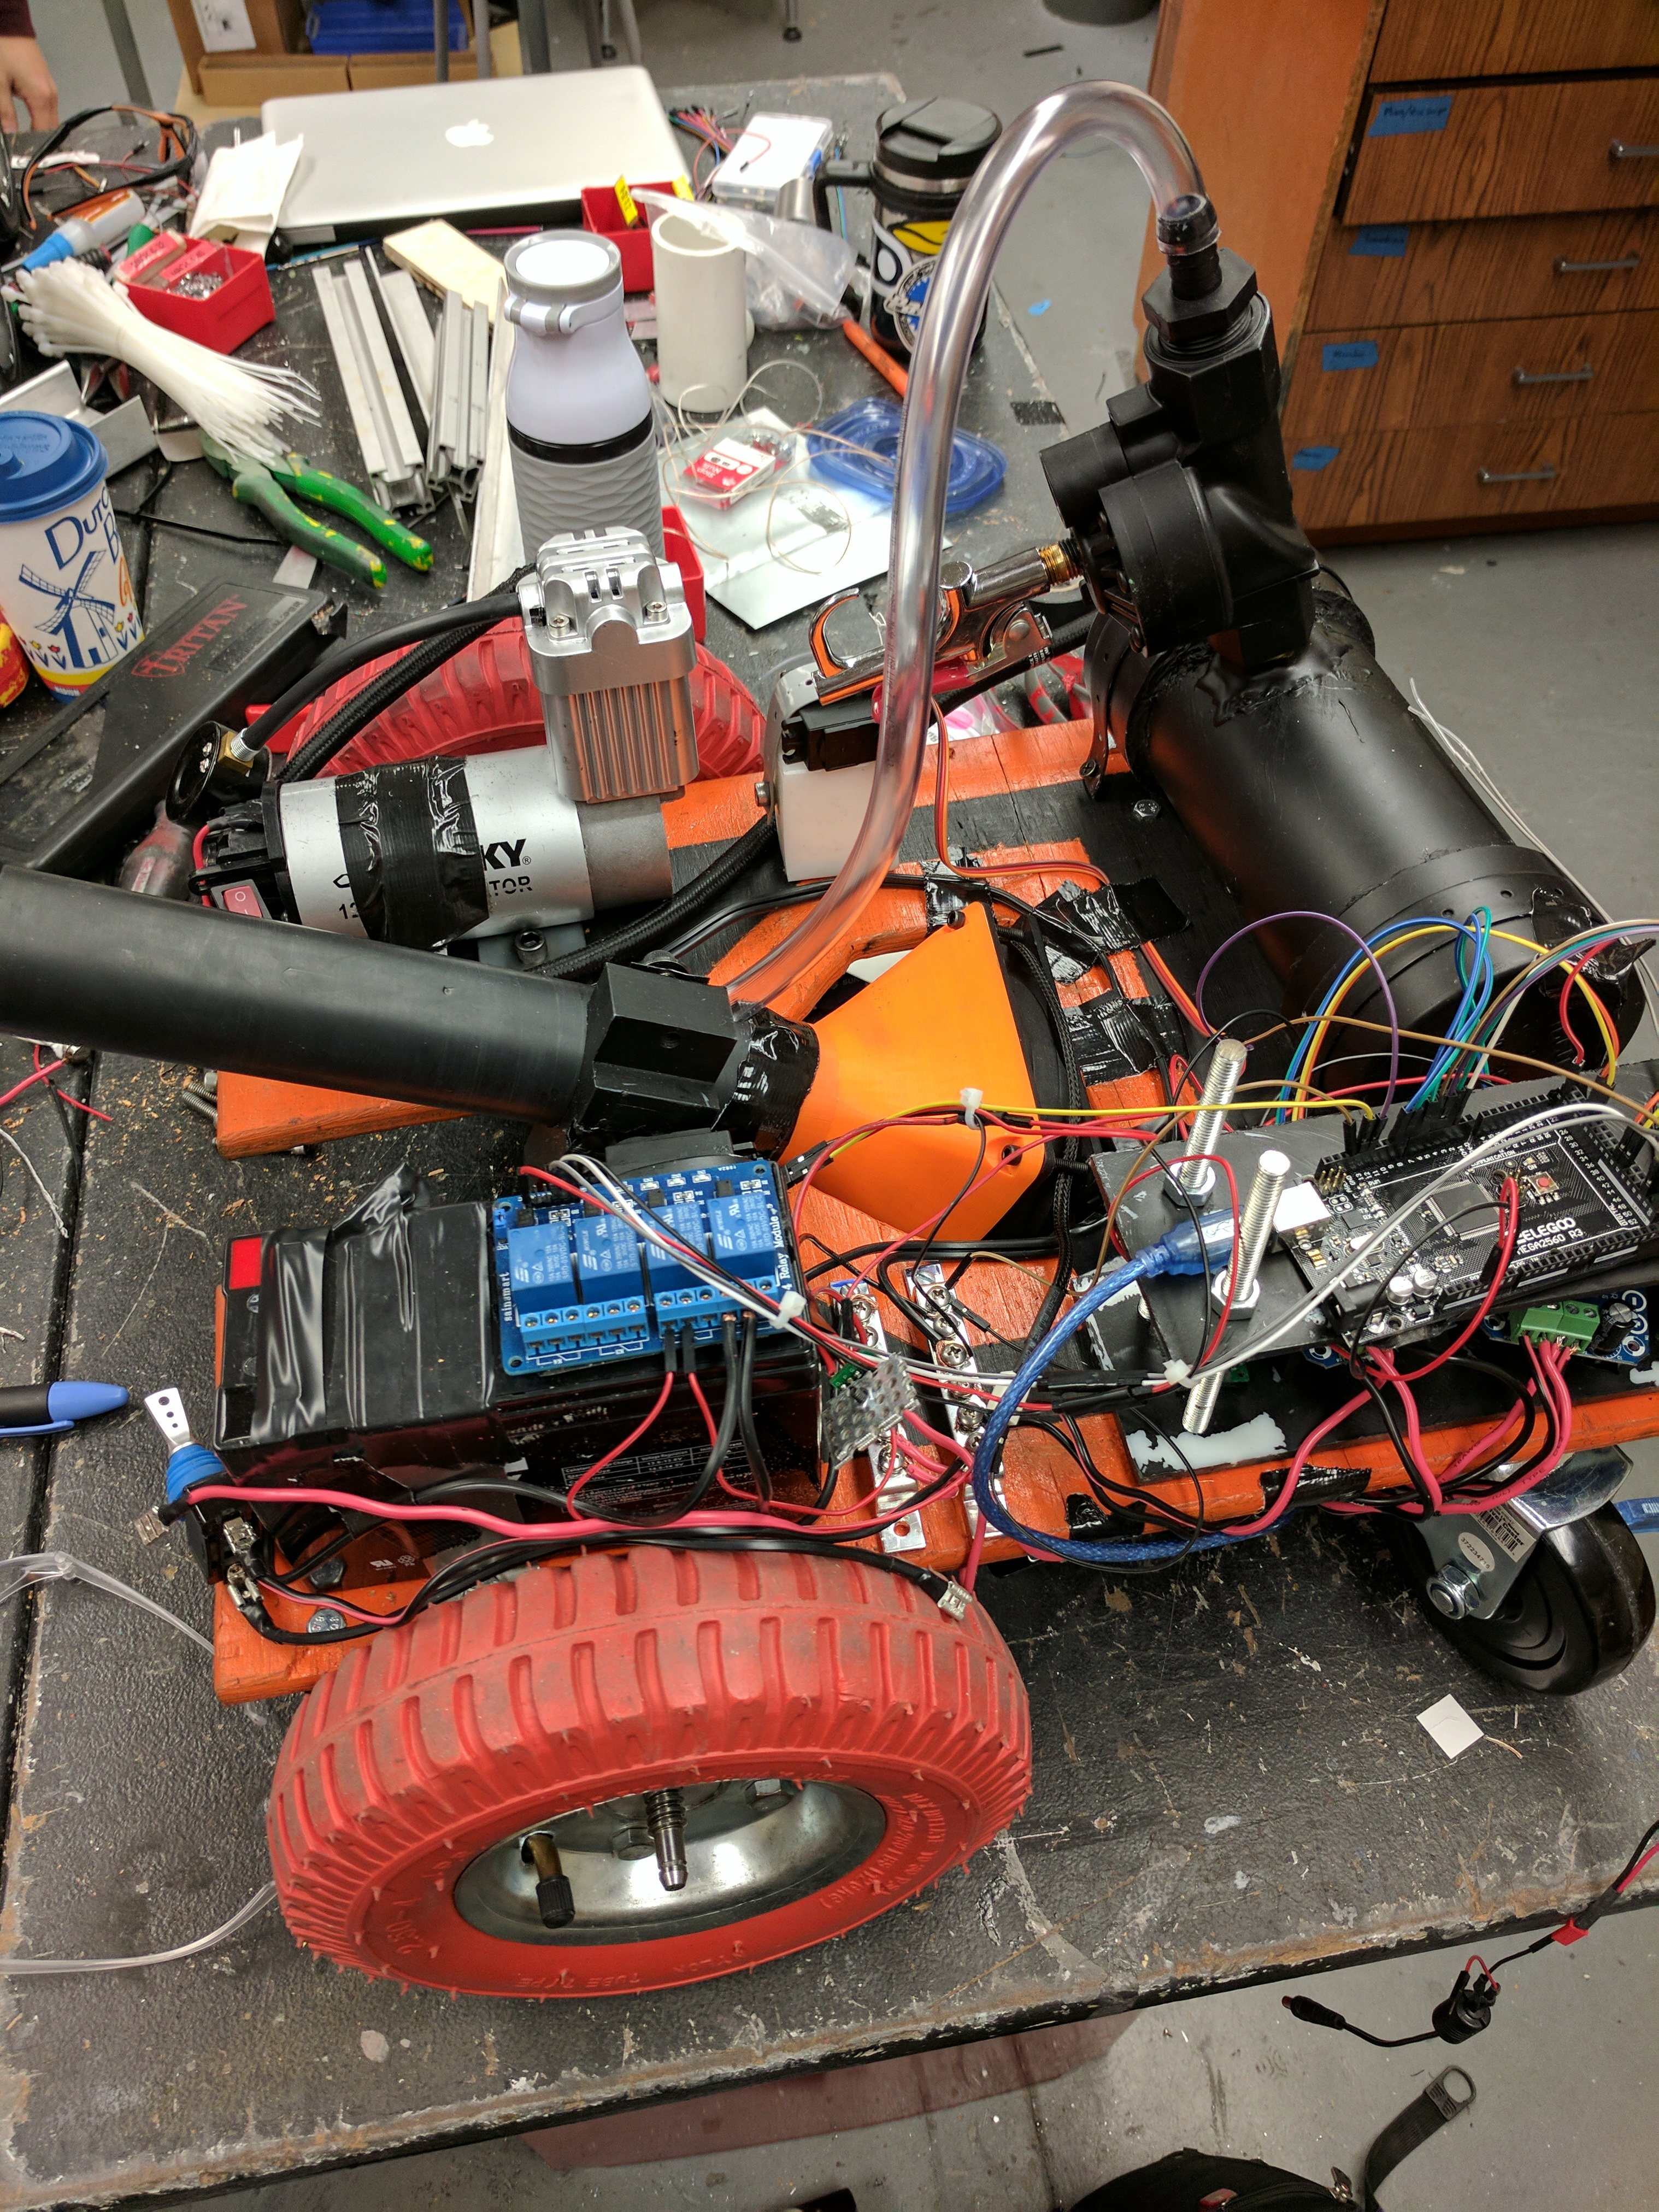
\includegraphics[height=4.5in, width=4in]{images/product}
	\label{fig:product}
	\caption{The robot just after final assembly}
\end{figure}

\begin{figure}[H]
	\centering
	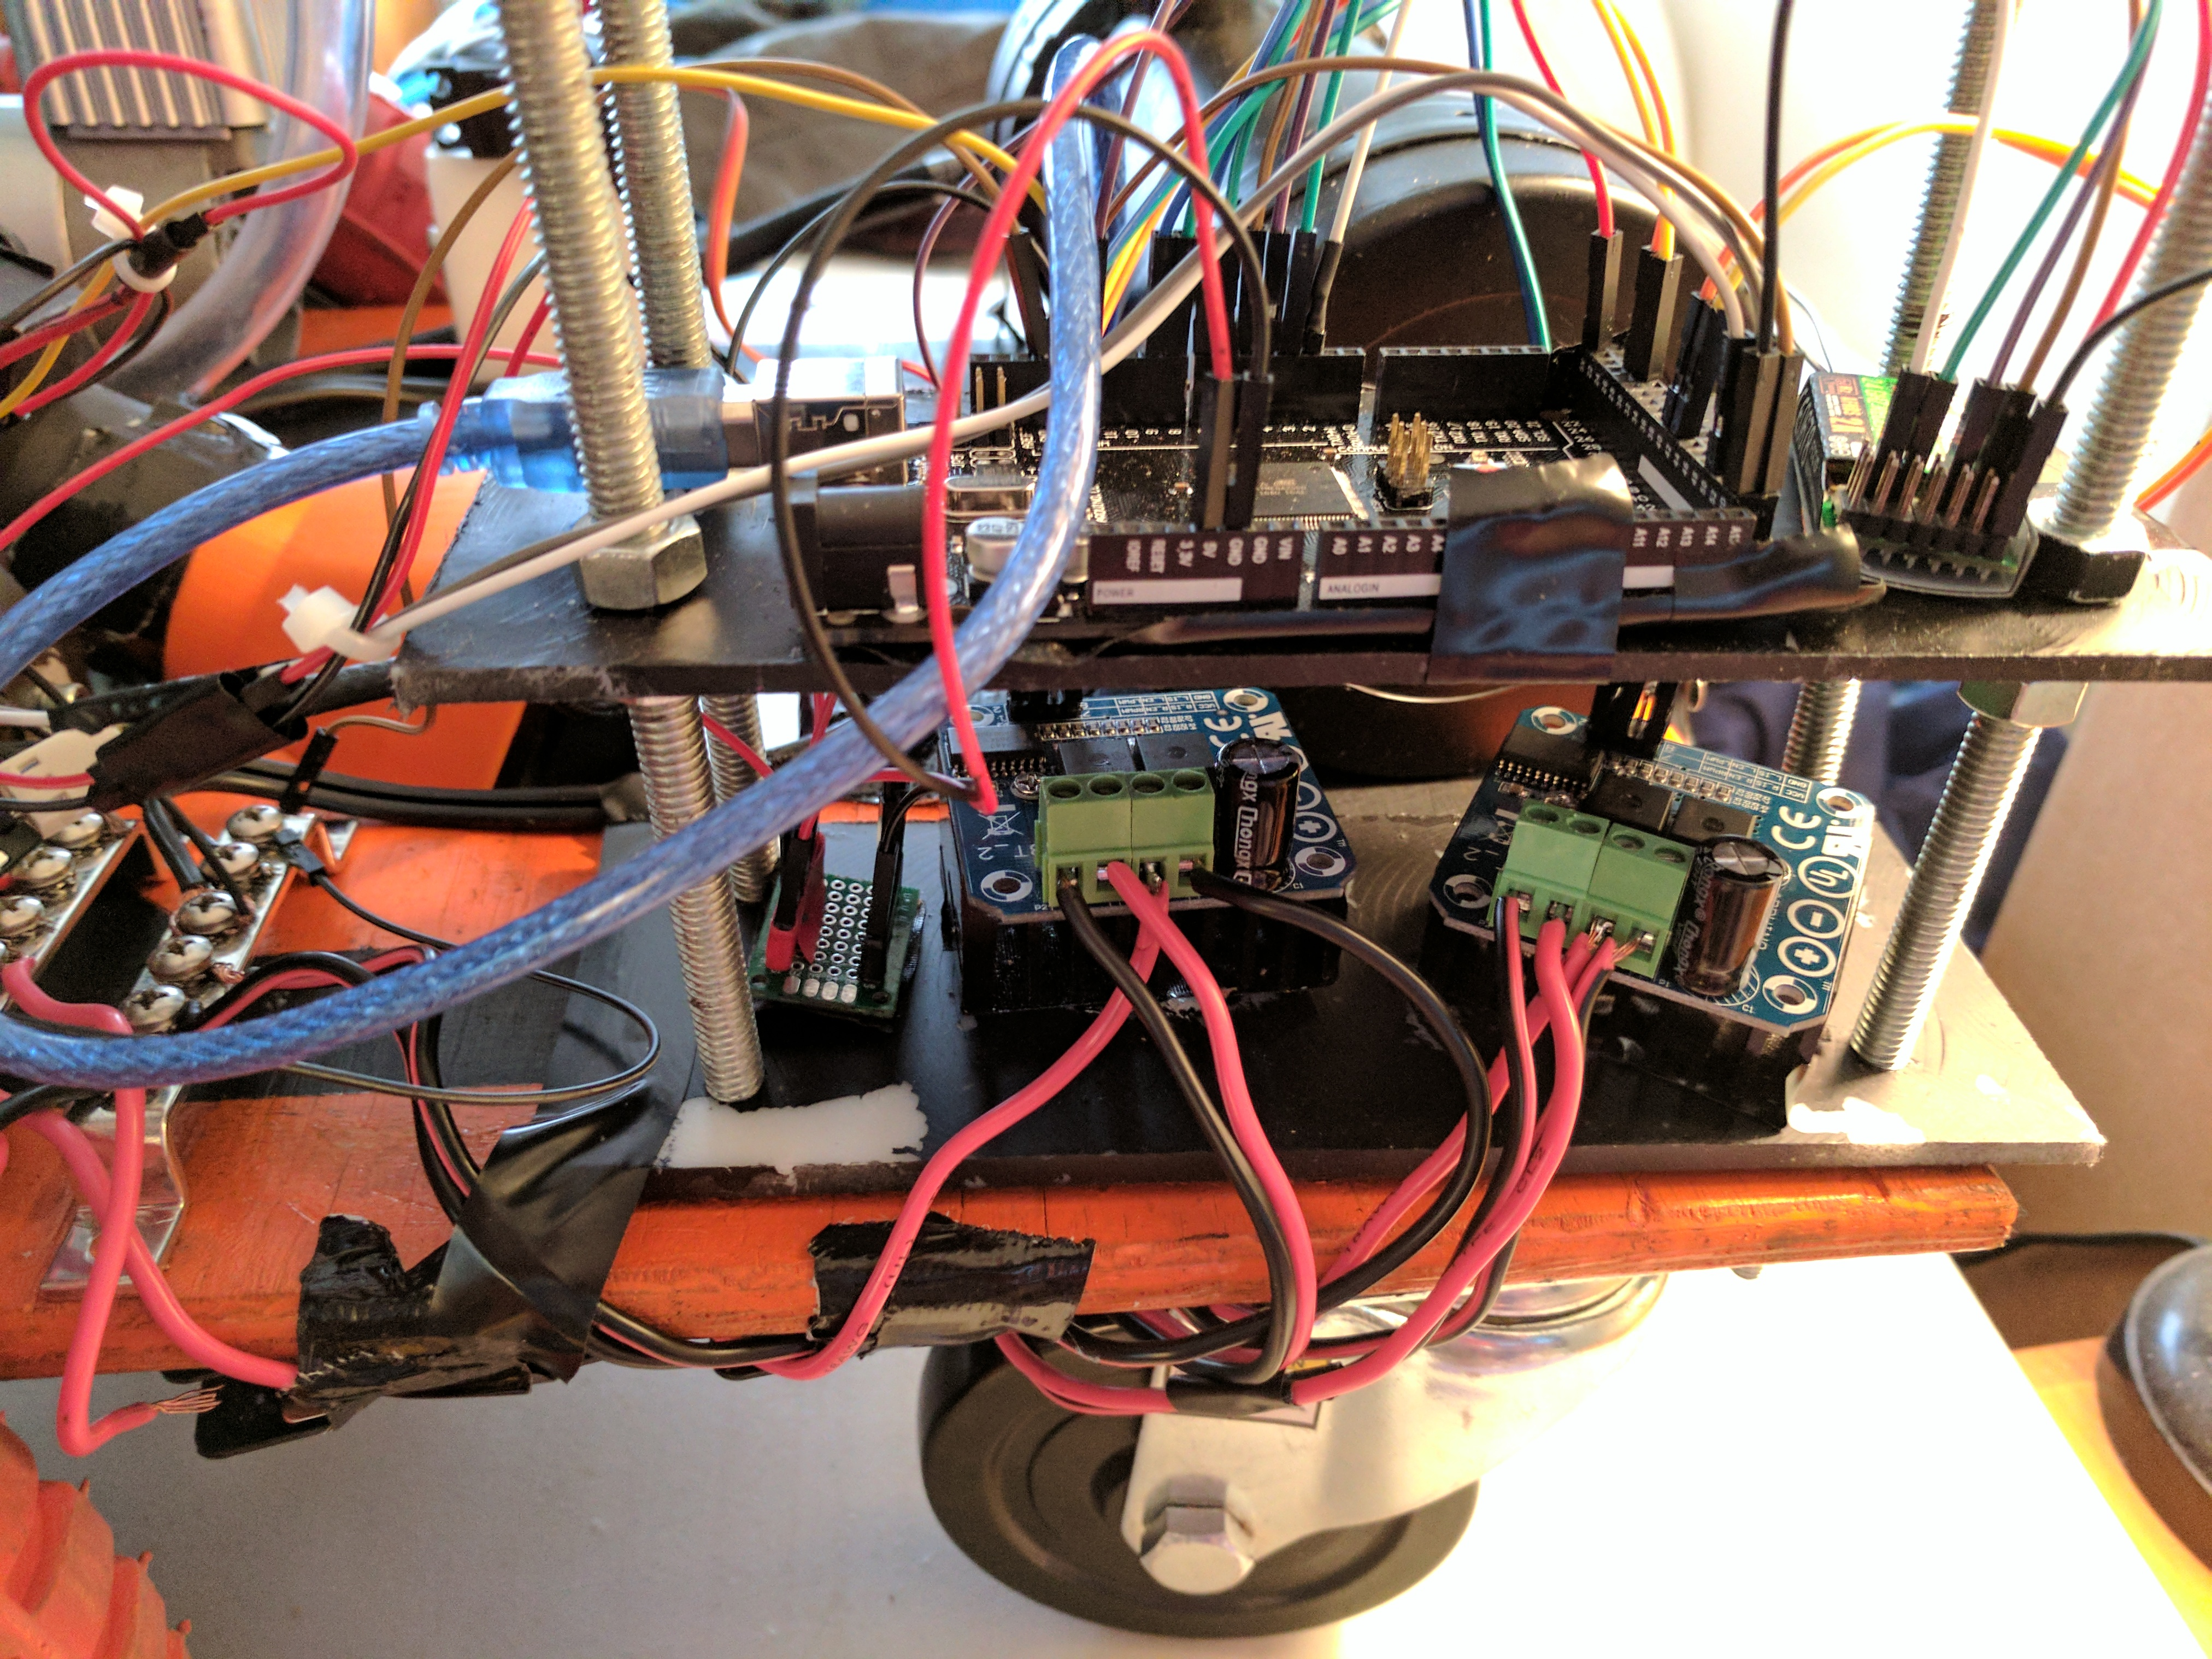
\includegraphics[height=3.8in]{images/circuit}
	\label{fig:circuit}
	\caption{Close up of the circuit}
\end{figure}

\begin{figure}[H]
	\centering
	\includegraphics[height=3.8in]{images/mount}
	\label{fig:mount}
	\caption{Close up of a motor mount}
\end{figure}

\begin{figure}[H]
	\centering
	\includegraphics[height=3.8in]{images/image2}
	\label{fig:chassis}
	\caption{Empty chassis with wheels attached}
\end{figure}

\begin{figure}[H]
	\centering
	\includegraphics[height=3.8in]{images/image1}
	\label{fig:testcircuit}
	\caption{Testing the drive component}
\end{figure}

\section{Conclusion}
\indent This project was an extremely valuable experience for our group, in that it required us to follow the same standard steps that would be completed for a similar design project in a professional capacity. This project was an excellent introduction to the product design process and has prepared us well for future group projects that we will take part, both at Oregon State and after graduation. We started off the project with a lot of different concepts in mind, and had a good idea of what we wanted the robot to look like when we were constructing our project plan and House of Quality. This helped us to refine our ideas into functional assemblies that could still be improved if needed, since it was still early in the project. When we were assembling the robot in its entirety we found that our design was sound but complicated. This fact is illustrated in Figures 20 and 21 where the electrical components and circuit can be seen, the large number of electrical components required a large amount of circuitry that was difficult to troubleshoot if sub function assemblies of the robot needed to be improved after testing. Overall the project was a success, citing the goals of the Team Charter, we finished in the top ten for the competition and even though we have yet to receive a final grade for the entire project we are confident in our work and expect meet the second goal of the Charter. A few things that we all took away from this project is that every task will always take more time than you think so plan accordingly. Also, prototyping is crucial; especially fro this class. It's much easier to eliminate a concept variant if you know it doesn't work. We prototyped our pickup mechanism in week 2 with an old fan and some cardboard. The driving portion of the circuit was also prototyped early on. Furthermore, we believe that our robot was over engineered and could have been much smaller. This is most likely attributed to a lurking bias that we wanted the robot to be able to have functionality outside of the class. While this is not necessarily a bad thing, make sure that you do not lose focus on the scope of the project; do more only once the necessary is finished. 

%\section{References}
\pagebreak
\begin{thebibliography}{9}
	\bibitem{car seat motor}
	American Science and Surplus Car Seat 12VDC Gear Motor. (n.d.).  Retrieved March 20, 2017, from \url{https://www.sciplus.com/p/CAR-SEAT-12VDC-GEAR-MOTOR_49248}
	\bibitem{motor driver}
	Infieon Technologies, 2004 BTS7690S Data Sheet. Retrieved March 20, 2017, from \\
	 \url{http://store.alhekma4u.com/content/ICs/Drivers/BTS7960S.pdf}
	\bibitem{compressor}
		Husky Tools, 2012 \textit{12-Volt Inflator, Use and Care Guide}. The Home Depot.
	\bibitem{Fan}
		Rosewill, Inc, "Rosewill RFA-120-K - 120mm Computer Case Cooling Fan." 2015. Web. 
	\bibitem{textbook}
		Ullman, David G., 2009 \textit{The Mechanical Design Process.} Boston: McGraw-Hill \\Higher Education, 2016. Print.
    
\end{thebibliography}
 
\end{document}